\documentclass[]{svjour3}
\RequirePackage{fix-cm}
\usepackage[utf8]{inputenc}
\usepackage[usenames,dvipsnames]{color}
\usepackage{fullpage}

\usepackage[numbers, sort, compress]{natbib}
\usepackage{graphics}
\usepackage{graphicx}
\usepackage{epstopdf}
\usepackage{color}
\usepackage{hyperref}
%\usepackage{pdfsync}
\usepackage{mdwlist}
\usepackage{colortbl}

\begin{document}

\title{Dynamic Application Runtime Environment (DARE): A
  Standards-based Framework For Building Science Gateways}

\author{Joohyun Kim \and Sharath Maddineni \and Mark Santcross \and Yaakoub El-Khamra \and Shantenu Jha}

\institute{Center for Computation and Technology, Louisiana State University, \email{jhkim@cct.lsu.edu} \and Center for Computation and Technology, Louisiana State University, \email{smaddineni@cct.lsu.edu} \and Center for Computation and Technology, Louisiana State University,  Bioinformatics Laboratory, Academic Medical Center, University of Amsterdam, \email{m.a.santcroos@amc.uva.nl} \and Texas Advanced Computing Center, TACC, The University of Texas At Austin, \email{yaakoub@tacc.utexas.edu} \and Center for Computation and Technology, Louisiana State University, Rutgers University, School of Informatics, University of Edinburgh, Department of Computer Science, Louisiana State University, \email{shantenu.jha@rutgers.edu}}

%\titlerunning{Dynamic Application Runtime Environment (DARE): A Standards-based Framework For Science Gateways}
%\authorrunning{Joohyun Kim et al.}

%\keywords{Science Gateways}
%\subclass{ MSC codes }
%\PACS{ PACS codes }
%\CRclass{ CR codes }

\date{Received: date / Accepted: date}


% \begin{center}
%   Joohyun Kim$^{1}$, Sharath Maddineni$^{1}$, Mark Santcroos$^{1,4}$,
%   Yaakoub El-Khamra$^3$, Shantenu Jha$^{1,2,5,6}$\\
%   $^1$ Center for Computation and Technology, Louisiana State University\\
%   $^2$ Rutgers University
%   $^3$ Texas Advanced Computing Center, TACC, The University of Texas At Austin \\
%   $^4$ Bioinformatics Laboratory, Academic Medical Center, University of Amsterdam\\
%   $^5$ School of Informatics, University of Edinburgh\\
%   $^6$ Department of Computer Science, Louisiana State University\\
% \end{center}


%\numberofauthors{3}
% \author{
% \alignauthor Joohyun Kim\\
%        \affaddr{Center for Computation and Technology}\\
%        \affaddr{Louisiana State University}\\
%        \affaddr{216 Johnston}\\
%        \affaddr{Baton Rouge, LA} \\
%        \email{jhkim@cct.lsu.edu}
% \alignauthor Sharath Maddineni\\
%        \affaddr{Center for Computation and Technology}\\
%        \affaddr{Louisiana State University}\\
%        \affaddr{216 Johnston}\\
%        \affaddr{Baton Rouge, LA}
%        \email{smaddineni@cct.lsu.edu}
% \alignauthor Mark Santcroos\\
%        \affaddr{}\\
%        \affaddr{}\\
%        \affaddr{}\\
%        \affaddr{} \\
%        \email{}
% \alignauthor Yaakoub El-Khamra\\
%        \affaddr{}\\
%        \affaddr{}\\
%        \affaddr{}\\
%        \affaddr{} \\
%        \email{}
% \alignauthor Shantenu Jha 
% \titlenote{Author for correspondence}\\
%       \affaddr{Rutgers University, Piscataway, NJ 08854, US  }\\
%       \affaddr{CCT, Louisiana State University}
% %      \affaddr{214 Johnston}\\
%       \affaddr{Baton Rouge, LA, 70803, US}
%      \email{sjha@cct.lsu.edu}
% }


  % An understanding of challenges and computational requirements of
  % the life-science applications suggests that the uptake of
  % distributed heterogeneous scalable HPC resources demonstrate its
  % effectiveness as an integral component of a wide-range of
  % life-science gateways. DARE science gateways comprise a user
  % access layer and middleware layers built upon Simple API for Grid
  % Application (SAGA) and the SAGA-based Pilot-Job (SAGA-BigJob)
  % capability.
\maketitle

\begin{abstract}
  The importance, impact and percentage of resources assigned to the
  life sciences is increasing at a rate that is probably greater than
  most other disciplines.  Gateways have proven to be very effective
  access mechanism to distributed HPC resources provided by the
  production cyberinfrastructure such as TeraGrid/XSEDE and in
  particular a very successful model for shared/community access
  models, however, there are missing capabilities and abstractions
  that enable the use of the collective capacity of distributed
  cyberinfrastructure such as TeraGrid/XSEDE, especially those that
  can be used to develop gateways in an easy, extensible and scalable
  fashion for both compute and data-intensive applications.  We
  introduce the SAGA-based, Dynamic Application Runtime Environment
  (DARE) framework from which extensible, versatile and effective
  gateways that seamlessly utilize scalable distributed infrastructure
  can be built for life-science applications.  We discuss the
  architecture of DARE framework, discuss how gateways can utilize the
  framework, and discuss representative life-science gateways --
  DARE-HTHP, DARE-NGS. We establish that DARE provides interoperable,
  extensible and simple framework upon which to build gateways in
  support of life-science applications.
\end{abstract}

%  This work is predicated on three important trends: (i) that the
%   importance, impact and percentage of TeraGrid/XSEDE resources
%   assigned to the life sciences is increasing at a rate that is
%   probably greater than other disciplines, (ii) that gateways have
%   proven to be a very effective access mechanism to distributed HPC
%   resources provided by the TeraGrid/XSEDE, and in particular a very
%   successful model for shared/community access models, and (iii) that
%   in spite of the previous two points there are missing capabilities
%   and abstractions that enable the use of the collective capacity of
%   distributed cyberinfrastructure such as TeraGrid/XSEDE, especially
%   those that can be used to develop gateways in an easy, extensible
%   and scalable fashion for both compute and data-intensive
%   applications. We introduce the SAGA-based, Dynamic Application
%   Runtime Environment (DARE) framework from which extensible,
%   versatile and effective gateways that seamlessly utilize scalable
%   infrastructure can be built for a life-science applications. We
%   discuss the architecture of DARE-based gateways, and particularly
%   life-science gateways -- DARE-HTHP, DARE-NGS, DARE-RFOLD, and
%   DARE-DOCK, that use the DARE-framework to support a wide-range of
%   life-science capabilities.


\newif\ifdraft
\drafttrue                                                                                        \
\ifdraft
% \newcommand{\reviewer}[1]{ {\textcolor{blue}    { ***Reviewer:     #1 }}}
 \newcommand{\jkimnote}[1]{{\textcolor{green}   { ***Joohyun:   #1 }}}
 \newcommand{\jhanote}[1]{  {\textcolor{red}     { ***SJ: #1 }}}
  \newcommand{\smnote}[1]{  {\textcolor{red}     { ***Sharath: #1 }}}
 \newcommand{\todo}[1]{  {\textcolor{red}     { ***TODO: #1 }}}
 \newcommand{\fix}[1]{  {\textcolor{red}     { ***FIX: #1 }}}
\newcommand{\yyenote}[1]{  {\textcolor{blue}     { ***YYE: #1 }}}
 \newcommand{\reviewer}[1]{}
\else
 \newcommand{\reviewer}[1]{}
 \newcommand{\jkimnote}[1]{}
 \newcommand{\smnote}[1]{}
 \newcommand{\jhanote}[1]{}
 \newcommand{\todo}[1]{  {\textcolor{red}     { ***TODO: #1 }}}
 \newcommand{\fix}[1]{}                                                                              
 \fi



% \category{D.1.3}{Software}{Concurrent Programming}{ Distributed programming/parallel programming} 
% \category{J.3}{Computer Applications}{Bioinformatics}

% \section*{General Terms}{Design,Measurement,Theory}

%  \keywords{Science Gateway, Runtime Environment, Distributed Computing, Simple API for Grid
%   Applications (SAGA), Pilot-Job abstraction, Data-intensive Computing}

\section{INTRODUCTION}

%\subsection{TeraGrid Usage by the life-science community}

The importance of computing in the life sciences has been well
appreciated. % An interesting corollary is that the rate-of-increase of
% computing resources devoted to the life sciences is increasing, and
% arguably is increasing at a rate faster than any other discipline.
In spite of fundamental limitations on the accuracy of the data, as
seen from Figs.~\ref{tg2007} \& \ref{tg2008} and Table~\ref{tg2011},
the trends are somewhat unambiguous: among consumed computing resources via TeraGrid (TG, now XSEDE), the NSF-funded nationwide Cyberinfrastructure (CI) started in 2001 and operated between 2004 and 2011 in the USA, the percentage devoted to the life sciences is already more than any discipline and the usage seems to be increasing, whether measured by number of cycles consumed, users or allocations~\footnote{It is
  difficult to provide such information in a consistent way as the
  total number of cycles available year-to-year varies, but also which
  discipline a proposal gets assigned to is somewhat random; thus many
  chemistry proposals, even physics proposals are likely to be
  biological in nature.}.

% The single largest community is the life-sciences community --
% including MD (25\%)... Get a break-down of the total usage of the TG
% by discipline and application type.


\begin{figure}
 \centering
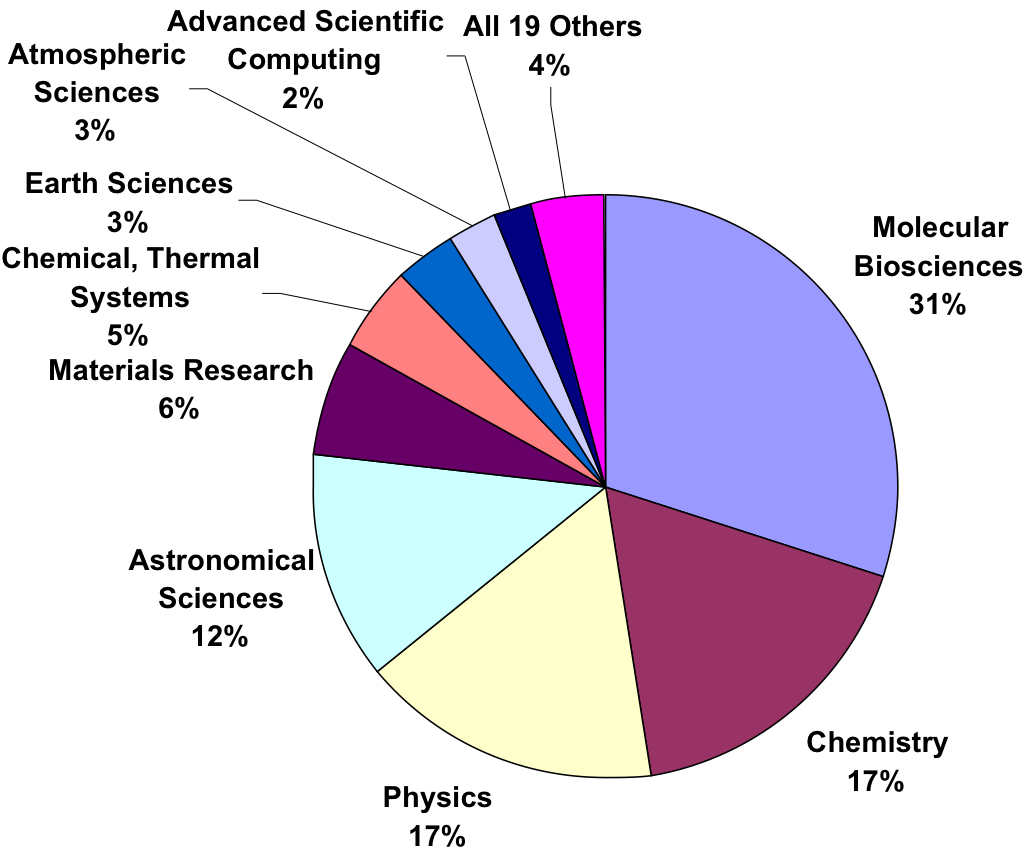
\includegraphics[scale=0.40]{figures/teragrid-discipline07}
\caption{\small 2007 Usage statistics for the TG. (Reference
  \url{http://www.teragridforum.org/mediawiki/images/9/90/II_WorkShop_G-HPC_Nework_2009-Towns.pdf})}
  \label{tg2007}
\end{figure}

With the exception of a few applications, e.g., large-scale
simulations (mostly Molecular Dynamics(MD) ) and virtual-docking
simulations, most life-science applications have not been very
effective in utilizing HPC cyberinfrastructure. Interestingly, MD
simulations have mostly relied on scaling-up to high core-counts,
whilst virtual docking represents a case beneficial with high-throughput calculations. However,
the need of large-scale distributed parallel execution for other
areas of biological/life-science applications is growing due to the
advances in experimental techniques producing large scale data sets with their high-throughput methods, as well as the advent of computing power and data management capacity. 

A specific example highlighting these trends and consequent challenges
arises in the context of Next-Generation DNA Sequencing (NGS)
technologies, with unprecedented amounts of data produced through
high-throughput methods and increasing computational requirements for gathering, management, and analyses of associated or produced data sets along a pipeline process. 

% for analyzing large volumes of data are
% effectively managed.

% required data analytics required
% along with dealing with 

Interestingly, the cyberinfrastructure (CI) considerations required to
support a broad-range of analytical approaches and at the scales
required, has received less attention than the data-management problem
and algorithmic advances. Thus not surprisingly, traditional
production cyberinfrastructure, such as the TG/XSEDE, have not been used for
such data-intensive analytics and distributed applications. There are
multiple reasons, but a couple of contributing factors are: (i)
insufficient runtime environments (and abstractions) to support
concurrent computational capabilities with large-data sets to support
data-analytics (beyond visualization) in an easy, scalable and
extensible fashion, (ii) insufficient support for user-customizable
data-intensive "workflows" that effectively hide the challenges of
data-movement and efficient data-management whilst managing concurrent
distributed (computational) resources.

It is interesting to note~\footnote{Based upon shared
  information/private communication between SJ and Dave Hart \& Dan
  Katz}: (i) Molecular Biosciences represented 25\% of TG/XSEDE (NU) cycles
used in Q1-2011. (ii) Based on the usage of the TG/XSEDE Science Gateways in first quarter of
20011, 3-4 of $\approx$ 20 TG/XSEDE gateways currently are biological/life
science, which in turn account for about $\approx$ 35\% of all gateway
usage. (iii) However, these 4 gateways account for about 2-3\% of
recording molecular bioscience usage. Points (i) - (iii) clearly imply
that although a significant fraction of TG/XSEDE cycles are devoted to
Molecular Biosciences (of which MD is the dominant component), very
few of the MD users actually use gateways to access TG/XSEDE resources.
Given the overall success and uptake of the gateways approach, prima
facie, there are reasons to believe that if a scalable, effective and
extensible capability were provided this {\it gap} could be overcome.
 
\begin{figure}
 \centering
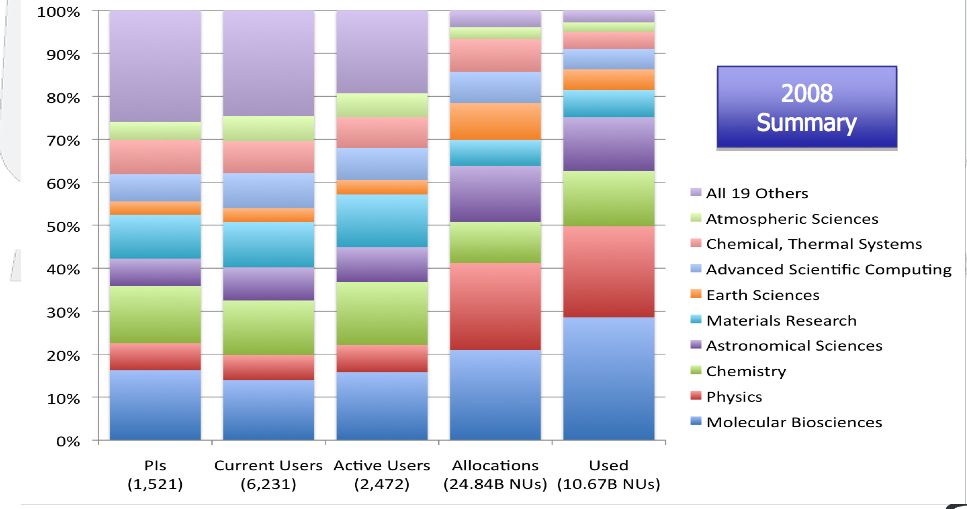
\includegraphics[scale=0.27]{figures/teragrid-discipline08}
\caption{\small 2008 Usage statistics for the TG/XSEDE (Reference
  \url{http://www.teragridforum.org/mediawiki/images/d/d8/DEISA-PRACE-May2009-Towns.pdf})}
  \label{tg2008}
\end{figure}

Science Gateways have witnessed impressive achievements in terms of the growth of the number of supporting
researchers and computing time usages\cite{gce11-nancy}. According to the very recent report about TG/XSEDE Science Gateway 
program\cite{gce11-nancy}, whereas, in 2006, 10 gateways consumed 100,000 CPU hours, in 2010, 22 gateways provided 40 
million hours usage and by 2011, nearly 40 \% of users on TG/XSEDE came through TG/XSEDE gateways. Interestingly, the CIPRES 
phylogenetic gateway, which was notably absent a few years ago, accounts for 25 \% of all TG/XSEDE users in 2011 exceeding 
other gateways dedicated to traditionally large-scale scientific computing domains, indicating a great potential of the 
gateway development for nurturing novel scientific computing practices and consequently for advancing associated 
scientific domains. 

Those gateway developments are often helped by suites of tools such as the Open Grid Computing
Environments\cite{ogce-2010}. However, most gateways do not support
distributed execution, i.e., most gateways still enforce the
tight-coupling between applications and a specific resource (see
table~\ref{table:TG-sg}). A primary reason is the additional, not
insignificant complexity to transform a target application to be able
to seamlessly utilize distributed cyberinfrastructure, and thus into a
distributed application.

We observe with the advent of federated grids such as TG and its
transition to eXtreme Science and Engineering Discovery Environment (XSEDE)~\cite{XSEDE}, such requirements
become harder to achieve as the number of connected sites and
heterogeneity will grow, as well as the computing power and the data
storage capacity of each resource reach peta or exa scales. More
importantly, supporting a broad range of diverse execution patterns is
critical considering different application usage modes for different
life-science applications. For example, in Table~\ref{table:four-applications}, the usage of four life-science
applications are summarized by contrasting conventional versus
distributed modes.
\yyenote{The following is a confusing sentence}\jkimnote{I tried to change it}
  Last but not least, it is always challenging to integrate effectively new
applications, to implement distributed data management with newly added infrastructure, and to introduce
a novel execution pattern, which is often eased by
the development of a framework.


\begin{table}
\centering
 \small
\begin{tabular}{|c|c|c|c|c|c|} 
  \hline  Quarter & PIs & Current & Active & Allocations  & Usage\\
  & & Users  &  Users & (NUs) $\times 10^6$& (NUs) $\times 10^6$ \\ \hline
  Q3 2010 & 249 & 1,044 & 366 & 8,810   & 2,219  \\ \hline
  Q4 2010 & 254 & 1,040 & 356 & 11,720  & 2,658, \\ \hline
  Q1 2011 & 257 & 1,168 & 418 & 13,101  & 3,412\\ \hline 
\end{tabular} 
\caption{Life-Science usage of the TG/XSEDE over the recent
  quarters. The figures establish that both the  allocation and the
  usage of life-science applications is increasing at least in
  proportion to the increasing resource availability on the TG/XSEDE,
  if not faster.}
 \label{tg2011} 
\end{table}

\yyenote{The following is the same incredibly long 3 sentences rolled into 1 from the abstract. Needs a bit of change}
This work is predicated on three important trends: (i) that the
importance, impact and percentage of TG/XSEDE resources assigned to the
life sciences is increasing at a rate that is probably greater than
other disciplines, (ii) that gateways have proven to be a very
effective access mechanism to distributed HPC resources provided by
the TG/XSEDE (and in particular a very successful model for
shared/community access models); given the landscape of the future
distributed cyberinfrastructure, we anticipate the importance of
gateways will continue to increase, and (iii) that there are missing
capabilities and abstractions to enable the use of the collective
capacity of distributed cyberinfrastructure such as TG/XSEDE, especially
those that can be used to develop gateways in an easy, extensible and
scalable fashion for both compute-intensive and data-intensive
applications.

Our primary strategy for gateway development concentrates on the development of a runtime environment for Distributed Applications (DA). The goals of DA are interoperability, distributed scale-out,
extensibility, adaptivity, simplicity -- referred to as
IDEAS\cite{ideas}. For instance, previously, as a modest step towards addressing point (iii),
we have shown that a flexible Pilot-Job framework can provide the
ability to run many MD simulations effectively across multiple
resources on the TG/XSEDE~\cite{saga-royalsoc, saga-ccgrid10}. 
Specifically, we've shown how a SAGA-based implementation of the
pilot-job, supports the distributed application design objectives
categorized by the term IDEAS\cite{ideas}. 

In this paper we establish how these capabilities can be generalized
and provided via Science Gateways, to support a range of life-science
applications. We introduce the Dynamic Application Runtime Environment (DARE) framework that is built upon SAGA and establish its effectiveness as an integral component for life-science gateways by demonstrating that it can
effectively utilize the collective capabilities of distributed cyberinfrastructure such as the TG/XSEDE and LONI.

\begin{table}
\centering
 \small
\begin{tabular}{|c|c|c|c|} 
  \hline Gateway  & Type of & System  & Execution Mode 
  \\
  Name & Compu- & for a Typical & for Parallel/ \\ 
  &  tation & Task & Distributed \\
  & & & Computing \\  \hline \hline 
  
  CIPRES   & phylogeny  &  single node  & multiple  \\
   &  &   & independent   \\ 
  &  &  &  tasks \\  \hline
  GridChem   & quantum & single node or     & multiple  \\
     & chemistry, & small cluster & independent   \\
  & MD &  & task  \\ \hline
   GridAMP     & ASTEC  & legacy Domain  & pipelined \\ 
  & coupled with  &  Scientific Code   & HPC  \\
  & a parallel GE &   &  programs \\ \hline
  Nano  & portal  & large Set   & multiple \\
  Hub  & for nano- & of Tools  & independent \\
   & technology &  & tasks \\ \hline
  \hline
\end{tabular} \caption{Examples of existing TG/XSEDE Science Gateways. The list is not necessarily complete. More information including URLs can be found elsewhere \cite{tg-sg-list-url}. ASTEC means Aarhus Stellar Evolution Code.}
 \label{table:TG-sg} 
\end{table}


\jhanote{Need to talk about LifeScience Applications on OSG and EGI,
  i.e., generalise from XSEDE}

\section{THE CASE FOR COMMON FRAMEWORK TO BUILD SCIENCE GATEWAY FOR
  LIFE-SCIENCE APPLICATIONS}

% \jhanote{Should we bring this down to two?}

\begin{table}
\centering
 \small
\begin{tabular}{|c|c|c|c|} 
  \hline Science  & Supported  & Conventional   &   Distributed
  \\
  Domain & Appli- & Application & Application \\ 
  &  cation(s) & Usage Mode & Usage Mode \\  \hline \hline 
  
  Molecular   &  \texttt{NAMD} &  MPI-based  & ensemble-based   \\
  Dynamics  &  & single simulation  & multiple  \\ 
  &  & run &  simulation  \\ 
  &  &  &  runs \\ \hline
  RNA   & \texttt{SFOLD}, & short single task    & large number  \\
  Folding   & \texttt{RNAFold} & or a few serial & of tasks using   \\
  Prediction & &  tasks &distributed \\
  &  &  &   resources  \\ \hline
  NGS data     &  \texttt{BFAST} & memory-intensive  & data-intensive\\ 
  analytics  &  &  single-node   &  distributed  \\
  & & execution  & computing \\ \hline
  Virtual  & \texttt{Autodock} &  many tasks   & many tasks \\
  Screening  &  & using a cluster  & using multiple  \\
  (Docking) &  &  & resources \\ \hline
  \hline
\end{tabular} \caption{Examples of life-science applications of interest and their usage modes.  Gateways were developed for these applications using the DARE framework}
 \label{table:four-applications} 
\end{table}

Here we describe the four scientific applications for which we develop
DARE-based gateways.

\textit{Large-scale MD simulations:} Over the past two
decades, the field of biomolecular simulation has exploded due to
increases in computational power and parallel codes, the emergence of
accurate molecular mechanical potentials or force fields and
improvements in the methods~\cite{adcock2006}. 
A continually growing body of researchers apply atomistic and
coarse-grained MD simulation methods to facilitate drug discovery,
perform advanced materials research, to design and understand
biomolecular and designed catalysts, and to provide fundamental
insight into molecular structure, dynamics and interactions.

In response to the perceived needs and importance of molecular
simulations, numerous high performance distributed memory parallel
codes have emerged in the past two decades (e.g., NAMD, CHARMM,
AMBER, LAMMPS,GROMACS, etc.), and many now can directly include
quantum representations. An interesting challenge in the MD community
is, along with continuing efforts that tackle more scalable molecular
systems with longer time trajectories using more powerful machines, to
develop ensemble-based simulations over multiple HPC resources.

\textit{NGS genome data analytics:} In the past several years, with
the advent of NGS technologies~\cite{mardis2008-tig,metzker2010}, there
has been a major paradigm shift in biological/biomedical research.
The novel capability of cost-effective resequencing, full-scale
quantitative transcriptomics, and a holistic approach for cell
development and cell differentiation using protocols such as RNA-seq,
and ChIP-seq, opens a completely new era for life-science
research\cite{sorek2010}. 

In spite of such opportunities, the potential of current NGS platforms
is limited by the capacity to analyze the sequencing data generated
and the subsequent bioinformatics analysis and inference. Furthermore,
the continuing trend of reduction in sequencing costs will result in
greater volumes and a concomitant increase in the challenges of
management and analysis. For example, current NGS platforms produce
typically billions of reads that comprise a short sequence mostly less
than 100 base pairs\cite{alex2009} and can require tens of thousands
of hours of computing time to effectively analyze.

%no sign to see the end of influx of new tools considering continuous 

There are numerous bioinformatics tools for NGS data analytics, and
thanks to continued innovation in the technologies and algorithmic
advances in such tools, their number continues to increase. Thus a
development approach to provide these tools and capabilities in a
simple, extensibile way is important; gateways provide precisely such
a mechanism.

In the current implementation, we focus on the most important analysis
of NGS data, that is of the mapping of NGS reads on to a reference
genome. Soon, this analysis step will be extended to support a broad
range of other analytic capabilities, such as genome variation,
genome-wide association, comparative genomics, and other applications
for investigating biological processes in a living cell.

%\textit{RNA structure prediction and beyond:} Defying the old
%biological dogma, positioning RNAs as a genome information
%intermediate between DNAs and proteins, during the last couple of
%decades, the number of scientific observations found that RNAs were
%actively involved significantly in gene expression and
%regulation\cite{joyce1999}. %,amaral2008}.
%Now, with the well-known categories of non-coding RNAs such as miRNAs
%and riboswitches, in spite of their biogenesis that does not need to
%be translated into proteins, significant roles of RNAs are quite well
%recognized\cite{costa2009}.
%%ellington2007}. 
%Importantly, RNA functions by forming required structure(s), and the
%pattern of structure formation of RNAs are somewhat contrasted to
%proteins that are mostly folded into highly specific 3-D
%structure\cite{roth2009}. For example, riboswitches chose one of two
%alternative structures, in response to metabolite binding,
%consequently resulting in two different gene regulation stages, i.e.,
%turning on downstream gene synthesis or turning it
%off\cite{montange2008}. Therefore, RNA structure prediction has been
%the major area for RNA studies and noticeable progress was made
%recently for RNA 2D structure prediction as well as 3D structure
%modeling\cite{shapiro2007}.
%
%\textit{Drug Discovery via Virtual Screening strategies:} For small
%molecule drug discovery, virtual screening using a docking method has
%been widely utilized and an immediate requirement for massive docking
%calculations against a chemical database has been attempted by
%managing such many tasks using a local cluster, HPC cluster, grids,
%and clouds\cite{levesque2009,yim2010}. The nature of required
%application usage mode for virtual screening methods is a generic
%example of many task computing, implying that pleasingly parallel
%massive tasks carrying out a docking computation should be executed.
%In spite of such well-established protocol, the challenges in drug
%discovery finding putative inhibitors for target receptors are not
%resolved due to intrinsic difficulties with underlying
%physico-chemical models associated with the issues with scoring
%function, receptor flexibility, and docking strategy itself.
%Therefore, more computing power and scaled calculations by varying the
%parameters for virtual screening are needed in order to understand the
%accuracy of results, suggesting the need of scalable infrastructure is
%highly appreciated while the application usage mode is generally
%intact.

% \subsection{Computational requirements and challenges}

% A growing limitation of applications in the life sciences is that
% workflow, data management, and analysis have become rate limiting
% steps: what is missing is support for the end-to-end execution
% requirement of applications.

% In essence, the move from executing an individual task to
% \textit{large ensembles} of coupled/loosely/uncoupled tasks requires
% scientists to spend significant time on compute and data management
% problems, instead of core science. The quantitative shift (massive
% distributed parallel compute and data resources) implies qualitative
% change in the way how life-science applications are being served for
% scientific discovery.

% We also need to move to tiered sets of computational resources. For
% example, one can imagine running large ensembles of MD engines on
% tightly coupled parallel machines (like Ranger or Kraken) with
% real-time data streamed to separately running analysis and
% visualization resources (Lonestar, Spur), with on-the-fly monitoring
% to analyze convergence, interesting phenomena or problems. This also
% provides the means for possible steering, for example by spawning or
% stopping separate elements of the ensemble to sample more or less in a
% particular region of interest. In addition to real time monitoring,
% hidden correlations in the data require the saving of coarser grained
% simulation data on longer term (1-2 year) disk resources for further
% analysis and mining using less tightly coupled computational
% resources, and ultimately placing reduced and derived data sets
% seamlessly back to the campuses, archivers, and for public
% distribution. Not only does this support the need for diverse sets of
% computational resources, large-scale storage and data transfer
% requirements for sophisticated analysis and visualization, and
% high-bandwidth networking, it also drives the need for software tools
% that facilitate the complicated workflow management, that allow
% dynamic monitoring, starting and stopping of ensemble elements without
% losing access to the global communications fabric and local
% connections, and that provide the means for facilitating data
% management and analysis.

% In essence, the move from executing an individual task to
% \textit{large ensembles} of coupled/loosely/uncoupled tasks requires
% scientists to spend significant time on compute and data management
% problems, instead of core science. The quantitative shift (massive
% distributed parallel compute and data resources) implies qualitative
% change in the way how life-science applications are being served for
% scientific discovery.

% The quantitative shift (massive
% distributed parallel compute and data resources) implies qualitative
% change in the way how life-science applications are being served for
% scientific discovery.

% \section{DYNAMIC APPLICATION RUNTIME ENVIRONMENT (DARE)}


\subsection{Pilot-Jobs for Life-Sciences For Distributed Applications}
\jhanote{Mark, SJ}

Ultimately Pilot-jobs are about the separation of resource assignment and
workload management.


\section{DARE -- A Critical Abstraction: Providing a Common Framwork
  for Science Gateways}

Some recurring requirements of applications in the life sciences are
the need to support the end-to-end execution requirement of
applications, i.e., integrated workflow, data management, and
analysis. Additionally, more sophisticated execution modes are
required, e.g., move from executing an individual task to
\textit{large ensembles} of loosely-coupled or uncoupled tasks. The
need to support these requirements whilst making decisions about
scheduling, resources utilization, or workload partitioning etc..., at
runtime, make these dynamic applications.

Currently all of the above requires scientists to spend significant
time on compute and data management problems. To address some of
these requirements dynamically, and to provide the basis for
rapid development of gateways that are capable of utilizing
heterogeneous distributed computing resources in a scalable manner, we
develop the Dynamic Application Runtime Environment (DARE)
framework\cite{dareurl}.

In Fig.~\ref{fig:dare-arch}, we present the architecture of a gateway
based on the DARE-framework; it is comprised of the four layers : (i)
User Interface, (ii) Applications, Capabilities and Services, (iii)
Runtime Environment, and (iv) Resources. Note that this schematic
emphasizes primarily our own integration strategy around the layer 
L3, that is built with the DARE framework, to bridge resource
utilization and user interactions. Other aspects that
are required in a typical Science Gateway are not explicitly shown or
simply ignored.

Also, it is noted that the schematic shows clearly that underlying
development mechanisms are independent and modular, but effectively
connected to each other under the framework. More details will be
discussed later in conjunction with Science Gateway development.

The critical aspect of the DARE framework is powered by SAGA and
SAGA-based Pilot-Job capability, the SAGA-BigJob\cite{saga-ccgrid10}. 
%
%We will show how the combination of the open-source web application
%technology, the runtime environment to support the execution of
%distributed applications enables the effective and quick construction
%of lightweight, extensible, gateways that can utilize
%distributed cyberinfrastructure. 


We first briefly describe SAGA and a Pilot Job abstraction SAGA-BigJob. 
 


\subsection{SAGA}

% SAGA is an API that provides the basic functionality for developing
% distributed applications, tools and frameworks. The key
% advantages of the development using SAGA include, but are not limited
% to: i) to provide a general-purpose, commonly used yet standardized
% functionality, while hiding complexity of heterogeneity of back-end
% resources, ii) to provide building blocks for constructing
% higher-level functionality and abstractions, iii) to provide the means
% for developing broad range of distributed applications such as
% gateways, workflows, application management systems, and runtime
% environments. Interestingly, SAGA provides a simple way to support
% scripting for building distributed applications via python-binding.


SAGA: Standards-based Building Blocks for Scalable and Extensible CI:
A fundamental question at the heart of all scientific applications and
tools, is the question of how they can be developed so as to use as
broad a range of infrastructure as possible, without vendor or
middleware lock-in, yet with the flexibility and performance that is
required. This question assumes greater significance in the distributed
computing context, such as grids and clouds, where resource ownership,
software providers, run-time environment and users are more decoupled
than for most other modes of computing. The Simple API for Grid
Applications (SAGA) has been developed to address precisely this
question. SAGA\cite{saga_url} is an OGF Technical Specification that
provides a common and consistent high-level API for the most commonly
required functionality to construct distributed applications, tools
and frameworks to support distributed applications. The functional
areas that are supported by SAGA include job-submission, file transfer
and access, as well as support for data streaming and distributed
coordination. SAGA provides both a syntactic and semantic unification
via a single interface to access multiple, semantically distinct
middleware distributions.

It is useful to understand the key advantages of development using
SAGA. They include, but are not limited to: (i) providing a
general-purpose, commonly used yet standardized functionality, while
hiding complexity and heterogeneity of back-end resources, (ii)
providing building blocks for constructing higher-level functionality
and abstractions, and (iii) providing the means for developing a broad
range of distributed applications, and tools to support distributed
execution, such as gateways, workflows, application management
systems, and runtime environments.

Different aspects of SAGA appeal to different groups. SAGA is now an
Open Grid Forum (OGF) is a standard. The standardization is important
because it makes it more likely that production infrastructures, like
NSF XSEDE and Open Science Grid, will support SAGA, which will make it
widely available for users and developers of tools on/of national CI
projects. In fact as mentioned, SAGA is now part of the “official”
access layer for the \$121M NSF TG/XSEDE project[cite XSEDE], as well
as for the world largest distributed infrastructure EGI[cite EGI]. The
fact that SAGA is an OGF technical specification also makes SAGA
highly appealing to application frameworks, services and tool
developers, which is quite understandable, as it not only simplifies
their development but also makes for scalable, extensible and
sustainable development. Users find the simple and extensible interface
providing the basic abstractions required for distributed computing is
very appealing to add their own “functionality” to a core base of
functionality.

The SAGA API provides the base abstractions upon which tools and
frameworks that provide higher-level functionality can be
implemented. Ref.~\cite{saga_url} discusses distributed application
frameworks and run-time systems that SAGA has been used to develop
successfully. 

A prominent example of such a tool is the SAGA-based pilot-job – which
provides an interoperable pilot-job (see next subsection), with
consistent semantics and common usage across different middleware. The
SAGA-based pilot-job extends and generalizes the commonly used
Pilot-Job concept, and as a solid validation of the base standards and
abstractions that can be built upon them, has enabled applications to
use the same pilot-job API over hitherto disparate resources for the
first time; advantages include scalability, simplicity and
extensibility (of basic functionality). Similar advantages of
scalability, simplicity and extensibility are now being experienced by
Gateway developers as a consequence of DARE – a SAGA-based library for
developing Science Gateways.

A SAGA implementation consists of a high-level API, the SAGA
Engine providing that API, and backend, middleware/systems specific
adaptors, i.e., each of these adaptors implements the functionality of
a functional package (e.g., job adaptors, file adaptors) for a
specific middleware system. The engine is a dynamic library that
manages call dispatching and the runtime loading of the middleware
adaptors. Adaptors are also realized as dynamic libraries. The SAGA
API has been used (in C++ and Java versions) to provide almost
complete coverage over nearly all grid and distributed computing
middleware/systems, including but not limited to Condor, Genesis,
Globus, UNICORE, LSF/PBS/Torque and Amazon EC2.

SAGA is currently used on production CI in several ways: admittedly
the number of first-principle distributed applications developed is
low, but SAGA has been used to develop glue-code and tools that are
used to submit and marshal jobs \& data across and between
heterogeneous resources. Specifically, it has been used to support
multiple computational biology applications that use high-performance
and high-throughput molecular dynamics (MD) simulations. SAGA has been
used to develop a standards-based library for Science Gateways to
easily utilize different distributed resources; some science domains
that are using SAGA-based Science Gateways include gateways to support
next-generation sequencing, docking and high-throughput of ensembles.

\subsection{SAGA-based Pilot-Job}

SAGA-BigJob~\cite{saga-ccgrid10} was introduced as a general-purpose
pilot-job framework, with which various execution patterns and
application usage modes have been
supported~\cite{async_repex11,saga-royalsoc}. Previously, we
demonstrated how SAGA-BigJob was able to execute scientific
applications categorized as pleasingly parallel applications and
loosely coupled applications on scalable distributed
resources\cite{jha2009developing, ecmls10, ecmls11}

Using SAGA and SAGA-based frameworks to build gateways enables the
fundamental design objectives (IDEAS) to be met efficiently and
effectively.

\subsection{DARE: A high-level abstraction to support execution
  patterns and dynamic execution} \jhanote{All}

{\it MapReduce etc..}

\section{Four Layers Architecture of DARE-based Science
  Gateways}

%\subsection{Four Layers Architecture of DARE-based Science
%  Gateways}

\begin{figure}
  \centering
  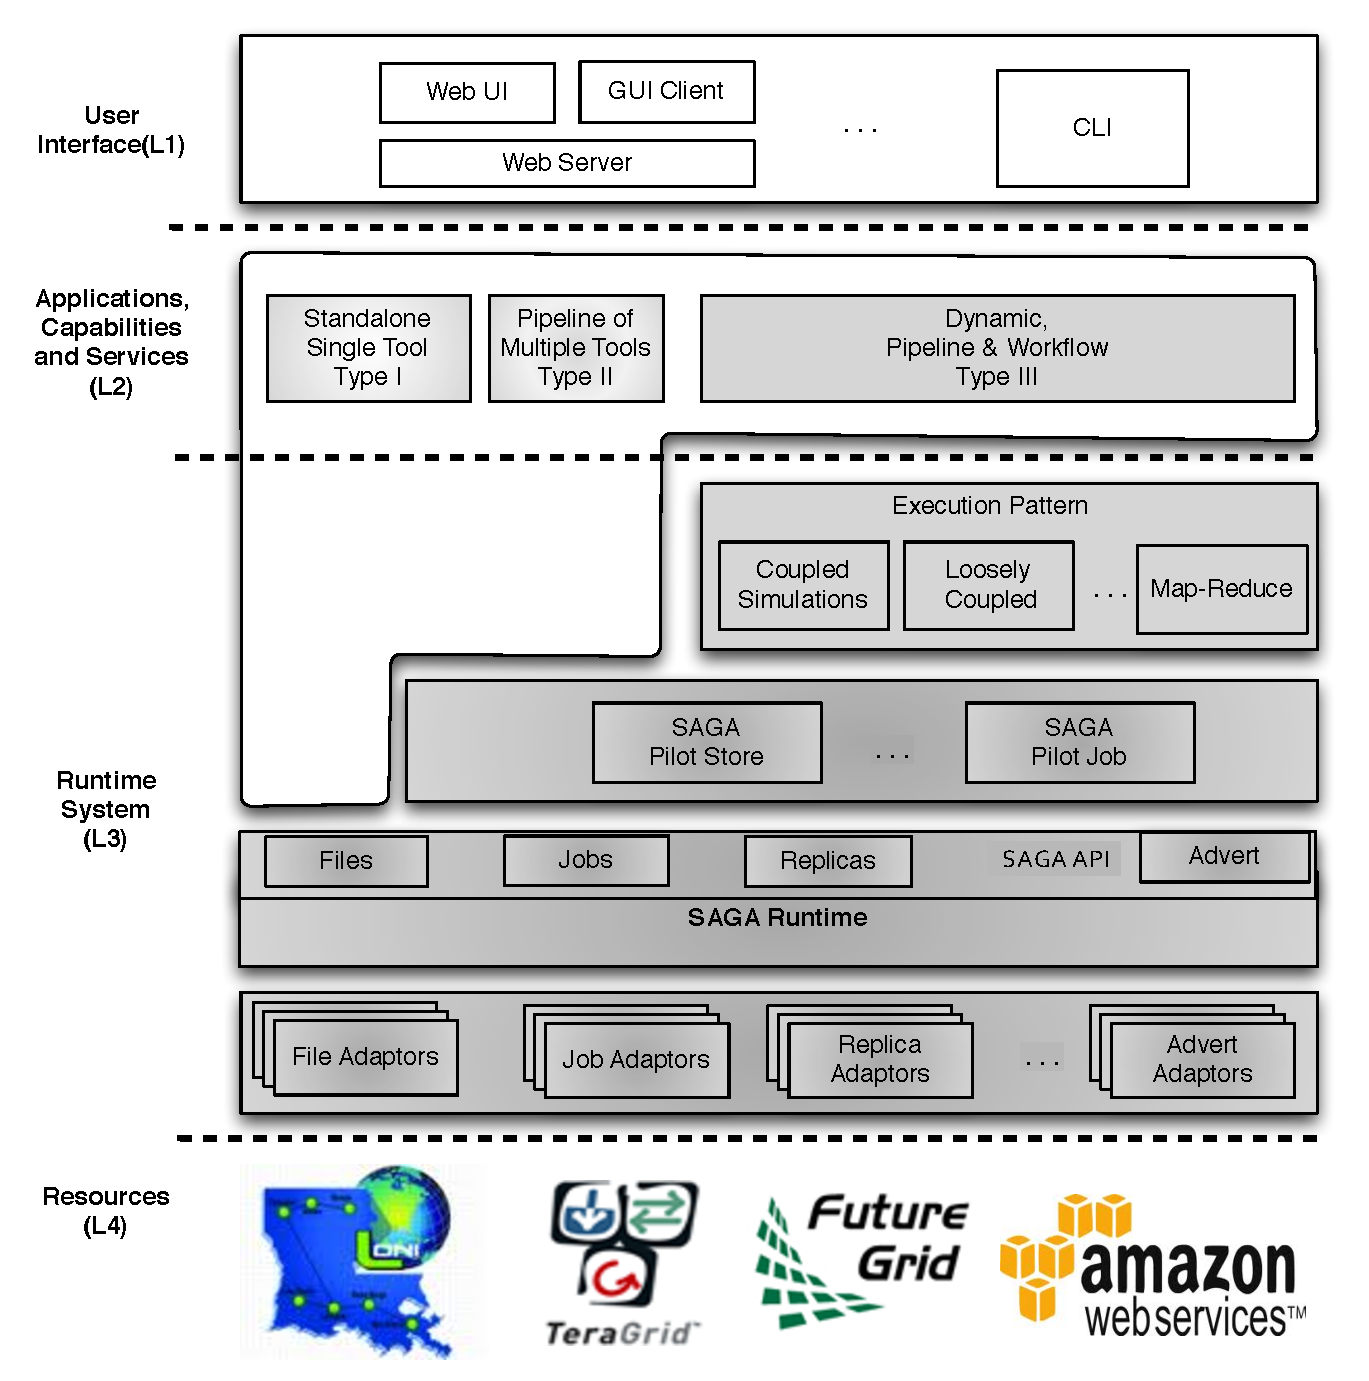
\includegraphics[scale=0.30]{figures/DARE-gateway-arch.pdf}
  \includegraphics[scale=0.30]{figures/DARE-gateway-alt.png}
  \caption{\small \jhanote{Use updated figure}(left) Overall architecture of a DARE-based gateway comprising four levels. (right) An illustration of a different view of a DARE-based gateway architecture}
  \label{fig:dare-arch} 
\end{figure}


As illustrated in Fig.~\ref{fig:dare-arch}, a typical gateway needs an access mechanism for dealing with user 
interactions including the authentication and authorization processes, middleware for carrying out user requests, job, 
and data management, and compute resources on which scientific applications are executed. 

\yyenote{The following sentence needs improvement: what do we mean by maximizing the capacity of DARE?}\jkimnote{i made a change}
One of our main design strategies of the gateway development suggested in Fig.~\ref{fig:dare-arch} is to maximize the 
strength of DARE for gateway applications.  The Middleware layers, L2 and L3, are decoupled from access level, L1, and 
resources, L4, and thus the development can enjoy the modular architecture. Additionally, the development and 
implementation of a broad range of execution patterns that are facilitated by pilot abstractions for distributed tasks 
and data are effectively achieved (which are the core features from DARE levels, L3) without knowing the details of high-
level characteristics of services that is solely defined in L2. 

\subsection{User Interface Level ($L1$)}
Depending upon the type of UI, i.e. Web-based or vanilla command line UI, three-tier or two-tier gateways are
possible. For example, if access mechanism is through a web browser or
a remote client, the overall architecture could be built as a three-tier
architecture in which a user desktop, a server that contains middleware comprising L2 and L3, and back-end resources
are independent to each other. Currently, the use of web
UI is a default for a user access. On the other hand, if
Command Line Interface (CLI) is preferred, the overall architecture would be two-tier, since there exists no need of a 
system for a remote user.   

The current prototype of DARE-based gateway architecture using Web-based UI is built upon the open source web application 
framework, pylons~\cite{pylonsurl}. Using pylons benefits primarily with its full-fledge web application framework 
capabilities allowing lightweight, extensible, and efficient web technologies, which is hardly achievable with other 
various Java-based approaches and other web application frameworks that might be more powerful but unnecessary 
heavyweight for tasks required for Science Gateways. Compared to them, pylons is widely proven with its efficacy for 
building a web application and high-quality features for a web application. 
The Model-View-Controller (MVC) architecture model that underlies the
pylons web application framework \cite{pylonsurl} is very effective and advantageous in
many ways. For example, database creation, management, and transaction
are extremely simple and robust to facilitate authentication steps and
job/data creation and management by storing or retrieving related
data. Additionally, UI creation/development and the connection
between server-side services (provided by the Services Layer) and
UI-based user interactions are also surprisingly simpler compared to
other existing approaches, requiring less programming efforts. For
example, it is well appreciated that for a science gateway
development, the utilization of databases and server-side programming
are non-trivial tasks. Finally, its python root is a plus factor that is easily integrated into the middleware including DARE core that are also written as python scripts.


\subsection{Applications, Capabilities and Services Level ($L2$)}

It is a developer's responsibility to find the optimal logic,
usage-mode for the target scientific application. The Application
Layer's role is to support this responsibility, i.e., implementing the
logic and usage-mode. Thus it is an important component of the
development and uptake of the gateway. As we will discuss, the
middleware Levels (i.e. L2 and L3) also mitigates developmental
hassles due to reliance on DARE, i.e. the SAGA/SAGA-based runtime environment framework.

The services provided by the gateway and their implementation of execution patterns and distributed modes for tasks and 
data are decided with L2. Note that the development of this level varies with target services, but could be efficient by 
abstracting various execution patterns and task/data management that constitute collectively the execution of dynamic 
applications. Such abstractions are implemented in L3 and facilitate the development of L2. Furthermore, we categorized 
into three kinds of services (Types, I, II and III), based upon level of complexity, scientists' usage mode,
and required software tools associated with the services provided via the DARE-based gateway, which provides the starting 
point of a target service with its general characteristics. In other words, this categorization also reflects 
characteristic features of such services with respect to execution patterns of tasks supported by DARE.

\begin{table}[!h]
\centering
\begin{tabular}{| l | l | l | l |} \hline \rowcolor[rgb]{0.8,0.8,0.8} &
Type I & Type II & Type III \\ Description & Standalone  & Pipeline & Pipeline \\ 
& Single Tool  & or Multiple Tools &  or Workflow-based \\\hline 
Target Tool Modification & Not Needed &
Not Needed & Minimally Needed \\ \hline Scientific Workflow & Not Needed & Useful but Not Necessarily &
Needed \\ \hline 
Example & BFast, BWA,  & MACS, TopHat-Fusion,  &   Novel Service for 
 \\
 &  Bowtie, ABySS  & TRANS-ABySS, Hydra & RNA-Seq \\
\hline
\end{tabular}
 \caption{Comparison of three kinds of services provided by the DARE-based gateway. }
\label{table:three-type-service}
\end{table}

Table~\ref{table:three-type-service} provides simple overview on the three types of services.

In brief, Type I \& II represent services that enable a user to run either as a standalone
application, an independent execution of multiple tools or pipelined
execution of multiple tools. Most of Tools in
tables~\ref{table:four-applications} and ~\ref{table:three-type-service} irrespective of their provisioning
as Type II/III are provided as a minimum as a Type I service.

A program developed as a single standalone application needs generally
less effort and is in many cases straightforward to integrate with
DARE; these are typically provided as Type I service. In contrast,
Type II services are built by incorporating different individual
tools/applications, and linked so that the output of one is
pre-determined as the input of another, i.e., provided as pipelines.

With the support using DARE, Type I \& II services have advanced features such as utilizing distributed
data-storage resources or distributed data management resources are available. In
general, all services will benefit from the seamless integration of
capabilities defined and supported in L3, e.g., pilot-job and
pilot-data abstraction from the L3 \cite{pstar11}.

Therefore, making a pipeline available as Type II services provides
two major advantages: availability of multiple tools that are used in
conjunction with each other in one location, and the enhanced
capability to utilize scalable resources such as TG/XSEDE and other HPC and
Cloud resources.

On the other hand, Type III services aim to support more complex
execution, both in the type of workflows supported as well as more
sophisticated execution. This is in contrast to Type I and Type II
services that aim to serve stand-alone and pipelined tools with advanced CI
capabilities -- scalable production infrastructure and integrative
efficient pipelines, but are limited for a static workflow implemented before the beginning of services.

Additionally, pipelines offered as Type II may often require greater
runtime flexibility, i.e., different stages may run on different
resources which may not be determined until execution time; these
``dynamic'' Type II pipelines will be thus offered as Type III
services. Thus the specific resources that are utilized in the
execution phase are determined dynamically -- either through delayed binding
or are refined/optimized after the initial resource assignment.

Type III Scientific workflows with dynamic execution are possible
with these DARE features. Type III workflows are fully customizable
and extensible, whereas Type II workflows are predefined and used as is.
Type III services obviously can run Type II workflows.

% To support these additional features, a Type III  scientific
% workflow with which a rapid development of dynamic execution
% patterns is possible. Workflows of Type III are customizable and
% extensible, whereas a workflow of Type II is predefined; Type III
% services can also invoke the ever-increasing concrete Type II
% services.

\subsection{Runtime System Level ($L3$)}
L3 represents the DARE and we describe here some backgrounds for its development and the relation with SAGA and SAGA-based pilot job abstraction, SAGA-BigJob. The challenges in building a scalable
distributed gateway is greatly mitigated by SAGA and/or SAGA-based
frameworks. For example, by varying SAGA-BigJob configuration, it is
easy to optimize the usage of target resources for a given
computational workload and their execution characteristics, such as
pleasingly parallel, loosely-coupled, or even multiple instances of
tightly-coupled applications. Thus once the desired configuration
has been determined, a gateway developer can easily construct
an optimized runtime environment for a given target application capable
of utilizing distributed resources in a relatively short development
cycle.

It is important to consider data movement requirements, since the
movement of large data sets such as input, output, and temporary files is
increasingly becoming a major challenge. We have recently analyzed the
date-volumes that need to be moved around, and demonstrated some of
the challenges and solutions (for the BFAST~\cite{ecmls11} -- as an NGS
application prototype). At the moment, GridFTP and scp are used as
the primary protocols for data
transfer. Table~\ref{table:NGS-Distributed-file} highlights the
significance of data transfer with data analytics for DARE-NGS with a
model system (human genome).

It is worth noting that SAGA provides different transfer protocols
as well as data-intensive programming models
such as MapReduce. SAGA also provides execution support for emerging 
data intensive computing infrastructure such as clouds~\cite{abstractions-azure,saga-ccgrid10}.
The DARE framework enables the simple utilization of these additional frameworks --
either as execution patterns or actual functional capabilities.

% This work presents four different gateways for different life-science
% applications, once 

% One figuring out preferable application usage modes as
% well as parallelization strategies, 

% The web interface will be connected to remote job submission via a
% job scheduling and monitoring thread. This thread starts with pylons
% application and continuously communicates with local database server
% to find new jobs and it also acts as a scheduler for new jobs. Once
% this thread finds a new jobs it will start preparing the
% configuration files for that particular job from the user and
% afterwords it will start the remote job submission via application
% specific SAGA-Bigjob.
%should be carefully considered when a gateway is developed,


% All the above components are well connected but loosely coupled from
% each others as well so this provides the development of different
% kinds applications very simple and fast.

\subsection{Resources Level ($L_4$)} 
While the utilization of distributed
heterogeneous resources should be one of the important motivations for a
science gateway development, most gateways currently rely on the
approaches in which multiple resource utilization is limited,
presumably, only for supporting pleasingly-parallel multiple tasks.
SAGA/SAGA-based frameworks enable distributed scale-out across
multiple production grade resources.

These production grade resources include grids of large systems such as Ranger, 
Kraken and Lonestar as well as HPC clouds on FutureGrid and vendor solutions such 
as Amazon's EC2. A basic design principle that the architecture adheres to is 
future-proofing through extensibility and abstraction. When adding a new 
computing platform, only a small amount of code has to be written as a SAGA 
adaptor to enable access to that platform.

Various SAGA adaptors contribute to achieve interoperability for
inter-HPC-grids, HPC-cloud, and other hybrid resources. There is also the
capacity to develop new developers complete with full documentation~\cite{saga_url}.
In addition, SAGA-BigJob adds the
capability to support various adaptive executions as already shown
with scientific applications such as Replica Exchange Molecular
Dynamics, hybrid CFD-MD, and NGS data
analytics~\cite{saga-royalsoc,coupled,ecmls11}.

It is important to note that SAGA is deployed in publicly accessible local 
installations on Ranger, Lonestar, Kraken, Steele and other XSEDE resources. SAGA 
is also a part of the software stack on FutureGrid machines. Furthermore, several 
virtual machine images with SAGA installations are available publicly on EC2. These installations are constantly updated, 
maintained and tested for quality of service and to detect any grid or cloud service outages.

% \jkimnote{the following paragraph needs to be shorten or moved into
%   the Services Layer?}  The access layer is connected to service layer
% with the help of configuration files. The job-scheduling/monitoring
% thread which starts along with the web server is responsible for
% writing the job configuration file which changes for every single
% job. Apart from this job configuration file there are two other
% configuration files, first one has the resource list which is common
% for any application (DARE-NGS, DARE-HTHP etc. ) and the other one is
% application specific configuration on each resource containing the
% paths for executables, input, output directories. once the
% job-scheduling/monitoring thread creates the job specific
% configuration file, it invokes another thread which starts reading the
% configuration files assigned to it and acts as a manager for this
% particular job. And this thread is responsible for transferring the
% appropriate input files to different resources, submitting and running
% the required jobs requested by user and getting back the output files
% which are in turn zipped and provided to user for download via
% web. But , we have keep in mind the uploading input files and
% downloading output file via web browser has not been implemented since
% the files sizes are too big to handle via browser and we are working
% on finding ways to handle this kind of situation. SAGA plays an
% important role with this job manager thread which makes the remote job
% submission and files/folders movement across different machines very
% simple and easily usable.

 \begin{table}
\centering
\scriptsize
 \begin{tabular}{|c|c|c|c|c|c|c|} 
 \hline 
Genome & Index         & Resource    & \# of & \# of &   \# of         &	TTC  \\
  Type               & File (GB)        & &Cores &   nodes &  VMs&  (sec)\\  
  \hline
 BG &0.435& R&	64 &4&-	&1067 \\
\hline                  
BG &0.435& QB	&	64& 8&-	&719 \\
\hline
 BG &0.435&R/QB	&	32/32 &2/4& -&919 \\
\hline
 BG &0.435& FG &	64 &-&8	&712 \\
\hline
 BG &0.435 &  R/QB/ &	24/24/& 2/3 & 3 &1022\\
 & & FG& 24 &&&\\
\hline
\hline
Chr &1.9& R	&	64& 4 &-&1145 \\
\hline
Chr &1.9& QB	&	64&8&-	&924 \\
\hline
Chr &1.9& R/QB	&	32/32& 4/2&	-&1170 \\
%\hline
%HG18-Chr21 &1.9& FG	&	64	& \\
%\hline
%HG18-Chr21 &1.9& R/QB/FG	&	24(2),24(3),	& \\
%&& 	 &24(3)&\\
\hline
\hline
HG &127& R	&	256 & 16 &-	&9586\\
%\hline
%HG &127& QB	&	256 &32 &-	& \\
\hline
HG &127& R/QB	&	128/128&8/16 & -&7582 \\
\hline
\end{tabular}
\caption{
  Comparison of Time to Completion (TTC) required for the NGS data
  mapping calculations using BFAST (match step) using DARE-NGS. 
  Three genome types,
  HG18 (HG), HG18-Chr21(Chr), B. Glumae(BG) represent a human genome,
  chromosome 21 of HG18, and the genome of a microbe Burkerholderia
  Glumae. Three compute resources are Ranger (R), QueenBee (QB), and
  FutureGrid  Eucalyptus Cloud on Sierra (FG), respectively. The
  number of tasks for carrying out the required mapping calculation is
  30(135MB) for B. Glumae and 32(169MB)for HG18 and HG18-Chr21.
}

  \label{table:NGS-Distributed} 
\end{table}

\subsection{Data Management in DARE-based Gateways}
\yyenote{This paragraph needs revisiting}
The two main features required for any science gateway are data management and task management systems. WIth the DARE framework, we aim to provide a solution for many challenges associated with such requirements, in particular in the context of the utilization of distributed heterogeneous resources. As mentioned earlier, the pilot job abstraction, SAGA-BigJob, has been successfully developed for distributed task management and integrated into the current DARE framework as a key component.  For data management, SAGA-BigData is being actively developed in parallel to BigJob. Nonetheless, the current implementation with DARE relies on the legacy approach for data management using file-based \yyenote{what does file-filed mean?}\jkimnote{it was a typo and corrected}, 
application-dependent implementation, and file transfer protocols using GridFTP and SCP are used as two main methods. Some 
benchmarking numbers for file transfer will be mentioned with the specific DARE-based gateway examples. 


\section{EXAMPLES OF DARE-BASED GATEWAYS FOR LIFE SCIENCES}

\jhanote{Some text here..}

\subsection{DARE-NGS}
The DARE-NGS gateway % (\url{http://dare.cct.lsu.edu/gateways/ngs})
is a prototype gateway built upon the DARE framework and focusing on Next-Generation Sequencing data analytics and downstream analyses; it currently supports the mapping
process using BFAST, BWA, and Bowtie and other pipelines for RNA-Seq and ChIP-Seq\cite{mardis2008-arghg,pepke2009}. Mapping (alignment) is the first
step in scientific discovery utilizing NGS sequencing-based protocols
including the whole genome resequencing, RNA-Seq, and ChIP-Seq. 

Recently, we investigated the mapping process using BFSAT, one of new generation alignment software tools. BFAST represents a software tool to aim high sensitivity rather than compute efficacy that is previously favored by popular aligners. It is worth mentioning that the computational complexity of the
analysis (e.g. mapping) depends, upon other things, on the size and
complexity of the reference genome and the data-size of short reads, but mostly algorithms\cite{ecmls11}.
Our investigation on computational requirements and efficient concurrency supports for data-intensive BFAST mapping led us to conclude that, given that these can vary significantly, the computational
requirements of NGS-analytics also varies (even between data-sets of
similar size). Thus an efficient, scalable and extensible analytical
approach must be supported by any framework supporting NGS-analytics.

%\begin{figure}
% \centering
%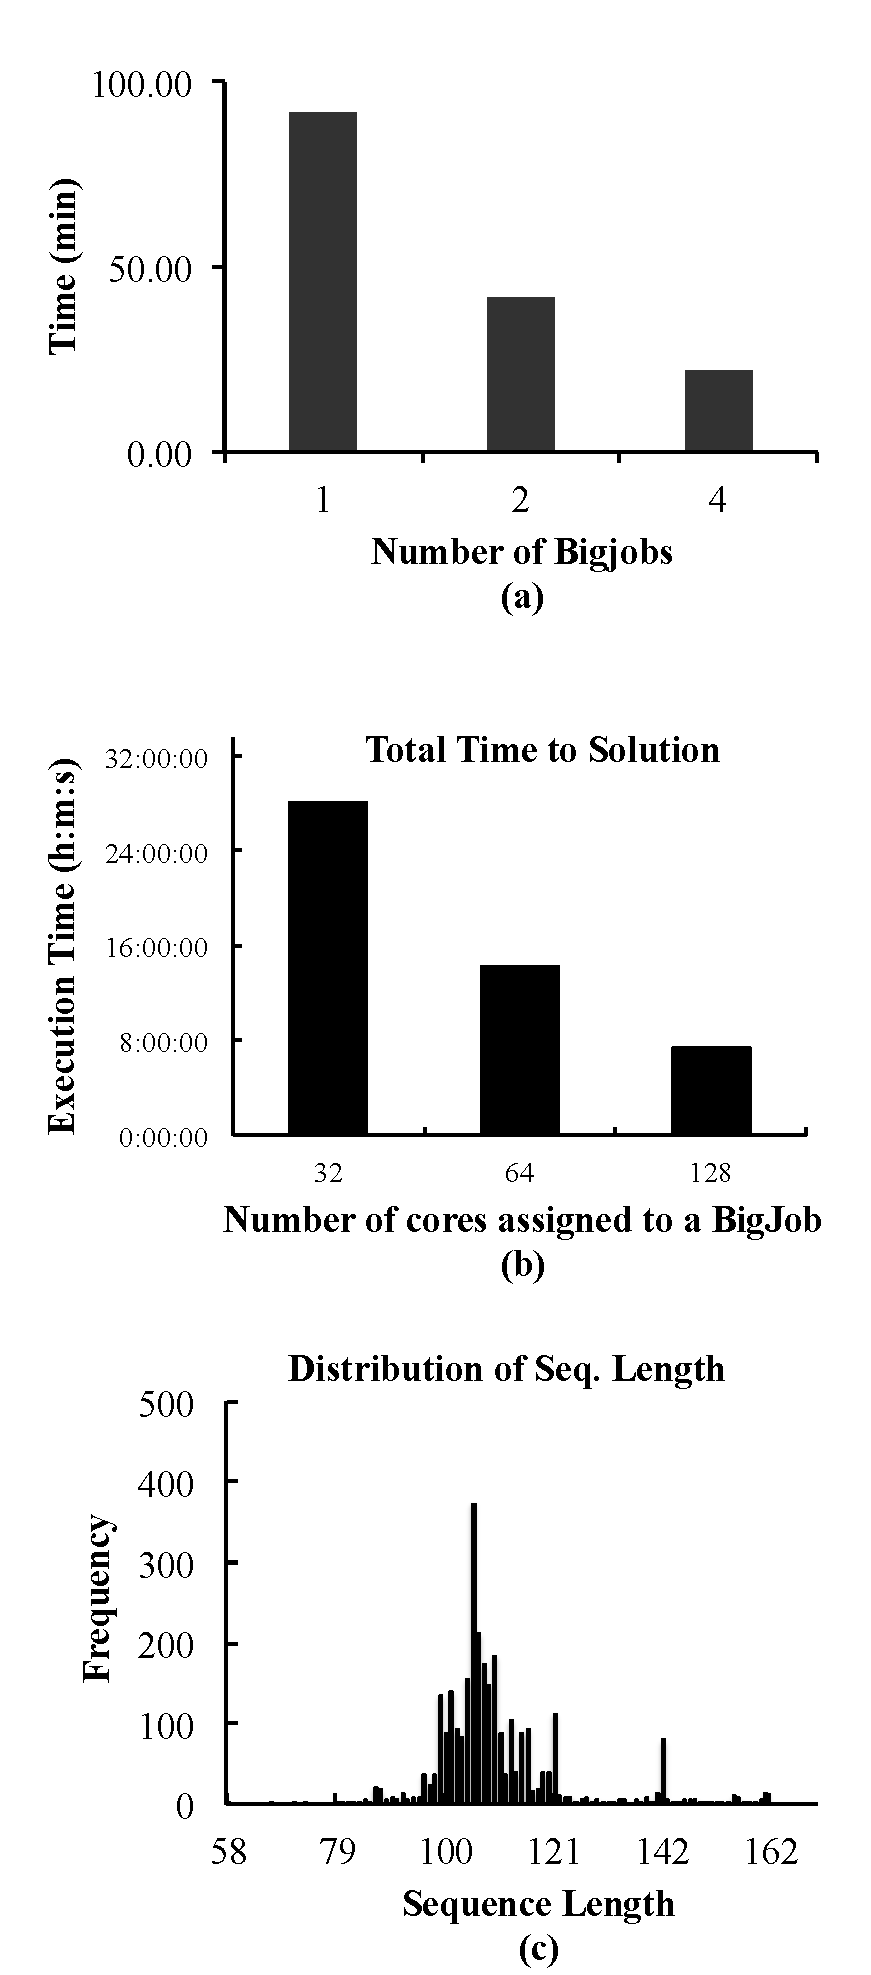
\includegraphics[scale=0.40]{figures/dare-rfold-result.pdf}
%\caption{\small Massive concurrent calculation capability is presented with the results obtained with DARE-RFOLD. The total 2910 SAM-I riboswitch sequences are injected into the DARE-RFOLD for sampling of Boltzman-weighted secondary structures. SAGA-BigJob handles these many tasks by decoupling the resource assignment and execution of each task, collectively allowing an efficient management of many tasks. In (a) and (b), time-to-solutions with different configurations of BigJob are compared in terms of the number of BigJobs (a) and the size of a BigJob (b). In (c), the distribution of sizes of 2910 input sequences is illustrated. This distribution is directly associated with the distribution of time-to-solutions of all 2910 tasks. The data are taken from the recent work\cite{ccpe11}.}
%  \label{fig:dare-rfold-result} 
%\end{figure}

The exploration of NGS analytics using DARE-NGS 
on HPC grids such as TG/XSEDE and Cloud environment of
FutureGrid were also conducted\cite{ecmls11}. Using the results obtained from such an
effort, we present the comparison of various execution scenarios with
multiple resources including a cloud system in
Table~\ref{table:NGS-Distributed}. While this demonstrates the
capability of DARE-NGS for utilizing HPC grids and a cloud environment
together or separately, our initial results, also, indicated several
issues with an emerging distributed environment. For example, we
observed that the large data management in FutureGrid clouds required
the Walrus data storage system but; however accesses through multiple VM's
often failed.

Such failures need to be managed, as human genome mapping requires
greater disk space than is often available in current (private) cloud
environments such as Futuregrid. Interestingly, we overcame some disk
space limitations, by implementing and exploiting task-level
concurrency. Nonetheless, gateway development should be flexible and
agile for future changes in resources and computing environments. Our works demonstrated that the DARE framework is an efficient tool for building a science gateway for sequencing data analytics and downstream analyses.

 \begin{table}
\centering
 \small
 \begin{tabular}{|c|c|c|c|c|c|c|c|c|} 
 \hline  
 	          & LW to QB (s)  & LW to Ranger(s) \\
 \hline                       
Avg. Rate && \\
MB/s & 112.04 $\pm 2$ &	    24.7 $\pm 2$  \\
 \hline                       
Index File	FTT & 1133  &	    5131.3      \\        
 \hline                       
Raw 	 Exome FTT&80.3 & 363.6\\                  
 \hline                       
Processed Short-&    & \\
Reads FTT&34&153.9  \\
 \hline                       
                    
\end{tabular}


\caption{Estimated File transfer times in seconds (FTT) with GridFTP between a local workstation (LW), QueenBee (QB), and Ranger with the case of Human Genome index files(127 GB), exome data (9 GB)and processed Short Read files (3.8 GB) . The high speed between LW (cyder located at LSU) to QB was because of the close spatial locality of the machines and LONI network which runs through LSU.  }

 \label{table:NGS-Distributed-file} 
\end{table}

Finally, for data-intensive computation such as NGS analytics, file transfer
processes are important for the total time-to-completion, and
Table~\ref{table:NGS-Distributed-file} shows such issues with the
measured transfer time obtained with DARE-NGS. At this moment, our
gateways employ GridFTP as a default protocol on the grids such as
/XSEDE/LONI and SCP for FutureGrid Sierra Cloud.



\subsection{DARE-HTHP}
\yyenote{Following sentence needs clarification}
An important challenge in modern biomolecular simulations, that has
received insufficient attention is to get single long-running jobs
completed, but managing and executing multiple instances of the same
(or similar) physical system. There are multiple reasons behind this
-- ranging from higher accuracy to reduced time-to-solution. For
example, multiple ensemble-member runs of the same physical system
enable better sampling In some cases, such as free-energy
calculations, multiple ensembles of the same system need to be
utilized. And even where a single long-running simulation is required,
thanks to algorithmic advances, such problems can be transformed into
the more {\it tractable} problem of solving multiple shorter run
simulations.



An ensemble simulation framework is required which has the following
characteristics: (i) Usable on a range of underlying distributed
resources and independent of resource-specific
middleware and services (i.e. scale-across), (ii) Efficiently manage
both scale-up and scale-out of ensembles -- possibly scaling up to
tens-of-thousands, if not millions of ensembles, with varying degrees
of coupling, (iii) Effective for a range of physical model sizes --
from thousands of atoms to hundreds of thousands of atoms, (iv) All of
the above without being tied to a specific underlying MD kernel, (v)
Extensible and Interoperable with emerging computational platforms
such as clouds. Our results presented in
Table~\ref{table:HTHP-Distributed} clearly show that DARE-HTHP is able
to run such an ensemble simulations.

\jkimnote{need the attention for the following. one or two sentence
  summary would be desirable}

%When the user submits the job to run on Futuregrid cloud environment
%the input files are transferred to different VM's. The configuration
%files that are prepared in the Access/Application layer will be used
%to launch the DARE Framework which in turn starts/submits according
%to the job configuration provided by user across Grids and Clouds.

To provide the capability to run jobs in cloud using DARE, we have
prepared images which have SAGA and other required adaptors installed
along with NAMD and MPI as well. These images are used to launch
multiple VM's and job submission similar to grid environment. Furthermore,
we are in a process of proving a capability where a user can upload
their images, and DARE will transfer them to Eucalyptus cloud on
Futuregrid and run on virtualized environment; it is also responsible
for marshaling the VM's and tasks in these environments.

 \begin{table}
\centering
\small
 \begin{tabular}{|c|c|c|c|c|c|c|} 
 \hline 
 Number           & Resource    & \# of &  \# of     &     \# of     &	TTC  \\
of tasks                &     &  Cores    &nodes&   VMs  & (sec) \\  
\hline
8& R&	64	&4 & - &141\\
\hline                  
8& QB	&	64& 8 &	-&176 \\
\hline
4/4&R/QB	&	32/32 &2/4&-&151\\
\hline
8&FG	&	64(8) & - &8&414 \\
\hline
2/3/3&R/QB/FG	&32/24/24&2/3&	3 &384\\
\hline


\end{tabular}
\caption{Time to completion (TTC) for 8 tasks of NAMD (each running on 8 cores,
  irrespective of the underlying resources), run over different resources. The three
  compute resources are Ranger (R), QueenBee (QB), 
  and  FutureGrid  Eucalyptus Cloud on Sierra(FG), respectively. The
  data shows that DARE-HTHC has been run successively on Grids and
  Clouds concurrently.}
 \label{table:HTHP-Distributed} 
\end{table}


\begin{figure}
 \centering
 \fbox{

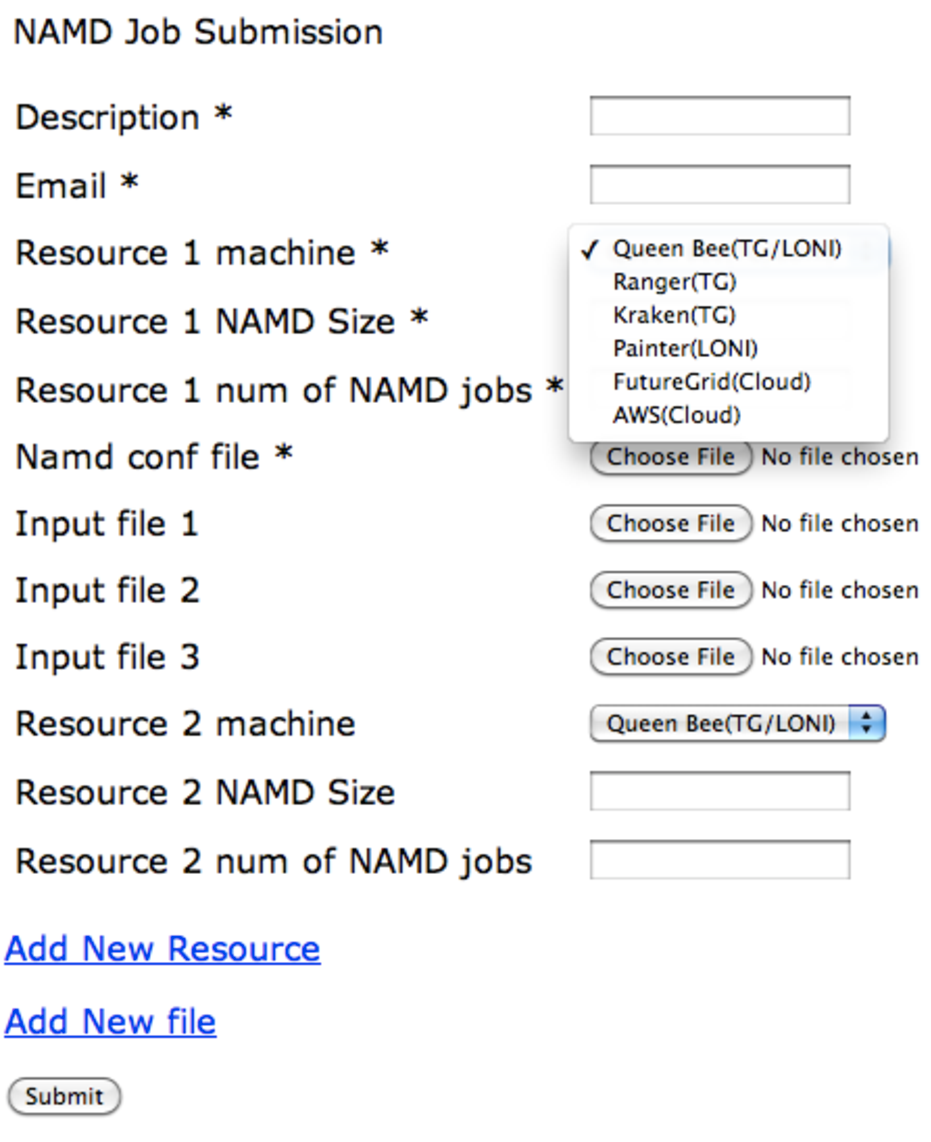
\includegraphics[scale=0.35]{figures/NAMD2.pdf}
   
  }
  \caption{\small \jhanote{Sharath: Need update figure} NAMD job
    submission web page form through DARE-HTHP. Here, the form
    indicates the usage mode with multiple resources. The simple case
    with a single resource is default, and a user can expands the form
    by adding more resources as shown. DARE-HTHP can be accessed at:
    \url{http://dare.cct.lsu.edu/gateways/hthp} }
  \label{fig:NAMD2}
\end{figure}


\subsection{Other Examples}
\subsubsection{DARE-RFOLD}
\yyenote{The following is a re-write. Please check}
We have been developing a gateway, DARE-RFOLD to support non-coding RNA research
and also to serve the RNA structure prediction. Through the DARE-RFOLD,
users can run simulations to predict the Minimum Free Energy (MFE) secondary
structure or run an ensemble of structures sampled with a Boltzmann-weighted
sampling scheme.

% To support nc-RNA research and broadly for the community who is
% interested in the utilization of RNA structure prediction for their
% research goals and education purposes, we have been developing a
% gateway, DARE-RFOLD, with which a user is able to predict the Minimum
% Free Energy (MFE) secondary structure or an ensemble of structure
% sampled with a Boltzmann-weighted sampling scheme.

Notably, our investigation into the computational requirements of RNA
folding dynamics suggested that the support of high-throughput
computation for a large number of tasks on heterogeneous distributed
resources is beneficial for the exploration of RNA folding energy
landscape and structural characterization of SAM-I riboswitch
sequences. As shown in recent works\cite{ecmls10,ccpe11}, the DARE
framework and its capacity for implementing a many-task-computing
support were demonstrated with the calculations of the total 2910
tasks needed for all well-known SAM-I RNA family with different
configurations for SAGA-BigJob set up\cite{ecmls10}.


\subsubsection{DARE-DOCK}
DARE-DOCK was developed for the basic virtual screening.  The current service with the gateway supports the docking with a popular application, Autodock\cite{autodock}. \yyenote{The following sentence is five sentences rolled into one. Needs work}\jkimnote{i chnaged}  Specifically, the docking calculation is carried out with the recently announced Autodock-vina, which allows to utilize fine-grain parallelism with multi-threading multi-core
support.  WIth such new capabilities with Autodock-vina, the gateway is able to carry out a very effective execution of high-throughput docking with multiple resources that is straightforwardly supported by DARE.  

%\begin{figure}
% \centering
%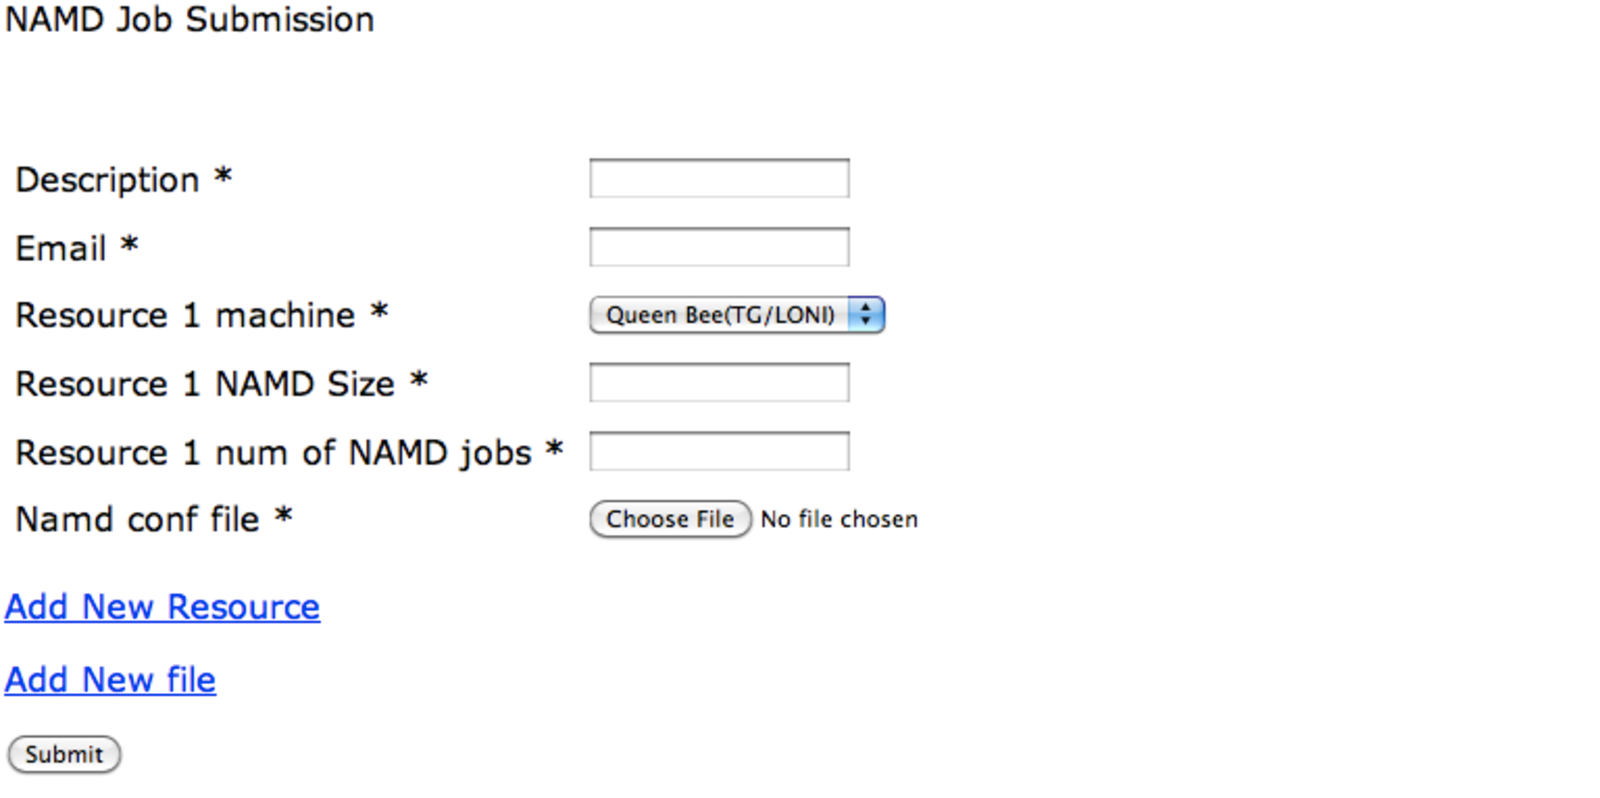
\includegraphics[scale=0.35]{figures/NAMD1.pdf}
%
%\caption{\small NAMD job submission web page form through DARE-HTHP} 
%\end{figure}

\section{Deploying DARE on TG/XSEDE}
\yyenote{The following is painfully obvious: of course we want to use XSEDE compute resources as compute resources, that is the entire point of a gateway. Way too redundant, I propose we remove.}\jkimnote{pleas make any changes if you want}
Nationwide cyberinfrastructure such as TeraGrid and its successor XSEDE, are increasingly playing an important role in 
large scale scientific computing. Similarly science gateways have been increasing in popularity.
With DARE, our effort to such a federated grid system are currently two folds. 
One is the use of large distributed HPC systems of the 
XSEDE program as resources for a gateway, and the other is to provide an entire gateway via XSEDE. 
For the former, the DARE-based gateways utilize the 'Community Software Area' which is a dedicated system space
managed and maintained by user groups, for providing domain or groups
specific software deployments. The SAGA software has been installed during the last year on all major TeraGrid (now 
XSEDE) machines, including Ranger, Kraken, Lonestar and others. The same mechanism is used to also provide SAGA on other 
infrastructures, most importantly on all FutureGrid machines.

The key benefit of CSA deployments on these XSEDE systems is that CCT's SAGA group is responsible for the SAGA 
installation and thus end users can focus on their own software built upon SAGA, and building a DARE-based gateway with 
XSEDE resources becomes efficient.

On the other hand, the second effort for providing a DARE-based gateway with XSEDE is to utilize Indiana University's 
Quarry system, which is a gateway hosting resource consisting of geographically
distributed Dell AMD systems that provide persistent, secure virtualization services.
Typically gateways would run natively on dedicated hardware that is
not directly connected (or affiliated) with XSEDE systems. With Quarry,
gateways can be run from gateway-developer run images hosted on an
XSEDE resource with high bandwidth connections to XSEDE HPC resources
as well as data repositories at TACC (Ranch), NCSA (Forge) and PSC (Albedo).

There are many advantages to virtualized gateway systems including
automatic nightly backups, quick restores (if re-deploying after failure),
reduced maintenance and so on. Furthermore, the virtualized solution has
low operational costs, high bandwidth and excellent support. There is however
a unique advantage to gateway framework developers: the ability to bundle
a VM image containing the gateway framework for immediate, user-ready deployment.
For DARE, the bundled image will contain the basic framework along with
demonstration web interfaces: DARE-NGS and DARE-HTHP. If a third party
user (or gateway developer) wants to use DARE, all users have to do is
run the DARE image on Quarry and setup their credentials.

By contrast, most XSEDE (and formerly TeraGrid) science gateways ran natively on hardware
with custom web and machine interfaces (https://portal.xsede.org/science-gateways).
Each of these gateways is a unique installation running on user side resources 
with custom scripts and more importantly custom interfaces to TeraGrid/XSEDE.
This complicates the deployment and utilization model of science gateways: each
gateway has to be a full ground-up development project and the entire development and deployment
burden is placed on the gateway developers.

The deployment and utilization model for DARE shifts the development and deployment
effort so that regular users (not necessarily gateway developers) can
get a basic science gateway running in quick order without much difficulty.
With a basic understanding of gateways, a user can start
their own DARE VM on Quarry and customize the existing building blocks
and interfaces to their satisfaction. This reduces XSEDE integration
overhead, gateway development and deployment overhead and unifies gateway
infrastructure for many applications. It is also important to note that
other XSEDE sites are in the process of deploying gateway hosting services
similar to Quarry, and with VM portability, DARE VM's can be ubiquitous on
these resources as well. Our expectation is to see science gateways as a
generic but customizable service available to users, complete with
building blocks in the form of ``canned'' virtual machine images.


\section{Conclusions}

All of the components in the DARE-framework are independent of each
other because to its modular design. The framework provides the key
functionality of job and data management over heterogeneous
distributed resources. This is provided so as to support various
execution patterns and application usage modes as well as the
full-functional access layer. Using this template, a developer can
quickly implement his/her own scientific logic in the application
layer with python scripts.

The objective {\it Distributed scale-out} is illustrated in
Table~\ref{table:NGS-Distributed}, where two large TG/XSEDE systems -- QB
and Ranger, were used for the match step in BFAST pipeline. As
demonstrated in numerous publications, having more resources and using
them collectively has multiple benefits, not least of which is the
decrease in the time-to-completion.

% It is
% noticeable that we compare different usage modes, for example, using
% one resource or two resource altogether with the same configuration
% for the computation. 

The results in Table~\ref{table:NGS-Distributed} also indicate there
are interesting aspects due to the complexity of scientific
applications. For example, for NGS data alignment using BFAST, one
needs to determine the optimal task-level concurrency based upon how
the reference genome indexes are utilized for chunks of short read
data\cite{ecmls11}. We have also used DARE-based gateways for
efficient scale-out of multiple MD simulations in different usage
modes.

% Not only have we
% established efficient distributed scale-out for data-intensive
% applications, we have shown the effective distribution of multiple MD
% simulations-- both in loosely-coupled and uncoupled ensemble-MD
% modes.

% While SAGA via the adaptor mechanism, provides the capabilities to
% expand the infrastructure it can be utilized on, e.g., t 

Extensibility is an important objective for DARE-based gateways, and
indeed, many levels of extensibility are easily provided and utilized.
The SAGA-based approach which provide numerous adaptors to different
middleware, supports interoperability across different middleware
types; it is limited only by the availability of adaptors (SAGA has
relevant adaptors to multiple existing infrastructure including
clouds). SAGA and SAGA-BigJob, combined together,
provide great flexibility to extend scientific capability of a
gateway, e.g., support of ensemble-based simulations as a primitive
``execution unit''. With DARE-RFOLD, we provided a pipeline whereby
% for another
% capability beyond RNA secondary structure prediction. We demonstrated
% recently that  
the output from the RNA secondary structure prediction
was utilized for Riboswitch gene annotation using structural
information. %  Furthermore, with the open source pylons framework,
% incorporation of web technologies is efficiently and easily achieved.

The design of the DARE framework supports adaptivity via the agile and
dynamic execution modes and the change of application usage modes
(e.g. concurrent multiple simulations to one large-scale simulation)
that the SAGA-based pilot-job provides.


% Note that not only varying the size of a BigJob, other possible usage
% modes supporting a case of loosely coupled applications~\cite{coupled}
% and a case of dynamically changing parallel/concurrent configurations
% in the fine-grain parallelization (for example, MPI configuration) as
% well as the coarse-grain parallelization are effectively designed.

Simplicity is provided by a well defined interface that supports
multiple {\it standards} distributed functionality, as well as
higher-level abstractions, e.g., based on the underlying SAGA-based
API, via SAGA-BigJob a general purpose Pilot-Job abstraction.

The new virtual machine image based deployment model on Indiana's Data
Quarry system enables rapid and hassle free deployment. No hardware
needs to be purchased, no backups arranged, and web development. In
due time, we expect to have popular content management systems with
DARE infrastructure available in images for the entire community to use.

In summary, we have demonstrated how providing the right abstractions
and easy integration with other components, enables DARE-based
gateways to support the effective and easy development of science
gateways that support distributed applications, whilst respecting the
IDEAS design-objectives. This includes novel data-intensive
life-science applications that utilize emerging distributed
computing/data resources such as TG/XSEDE and cloud environment
contributes.



\section{Acknowledgments}
This work is primarily supported and motivated by Grant Number
P20RR016456 from the NIH National Center For Research Resources. We
are grateful to Andre Luckow and Ole Weidner for their work for SAGA
and SAGA-BigJob development; we also thank Ole Weidner for a
constructive criticism of this manuscript and Andre Merzky for the information about SAGA CSA deployment. Computing resources used for this work were made possible via NSF TRAC award TG-MCB090174 and
LONI resources. This document was developed with support from the
National Science Foundation (NSF) under Grant No. 0910812 to Indiana
University for ``FutureGrid: An Experimental, High-Performance Grid
Test-bed.''. SJ would like to thank Dave Hart (SDSC) and Dan Katz
(Chicago) for helpful discussions.


%\bibliographystyle{spbasic}      % basic style, author-year citations
%\bibliographystyle{spmpsci}      % mathematics and physical sciences
%\bibliographystyle{spphys}       % APS-like style for physics

%\bibliographystyle{abbrv}
\bibliographystyle{unsrt}
%\bibliography{saga,tg11}
\bibliography{jogc,saga.bib}
\end{document}

% As we will show in \S4, building the DARE framework on SAGA and
% SAGA-BigJob, the fundamental design objectives of IDEAS, which
% constitutes essential requirement for distributed applications, are
% achieved in a remarkably effective way.

% -- Access/Application Layer, Services/Middleware Layer, and Resource
% Layer}
